\newpage
~
\section{Технологическая часть}

\subsection{Руководство по интеграции и настройке подсистемы}
Одной из целей при создании ПОАПО являлось создание удобного и простого в интеграции с другими системами модуля для автономной навигации объектов. Руководствуясь этой целью, процесс установки и настройки был максимально упрощен. 
Для корректной работы подсистемы необходимо использовать оборудование, указанное в техническом задании к системе, а именно:
\begin{itemize}
\item требования к цифровой камере:
	\begin{itemize}
	\item разрешение не ниже 1 Мп;
	\item интерфейс соединения со скоростью не ниже 12 Мбит/с;
	\item жесткое крепление на объекте;
	\end{itemize}
\item Требования к инерциальному измерительному устройству 
 	\begin{itemize}
 	\item трехосевой гироскоп с диапазоном измерения до 2000 $^\circ$/с и точностью не ниже, чем 0,2$^\circ$ на 1 $^\circ$/с;
	\item акселерометр с тремя степенями свободы и диапазоном измерения $\pm10g$.
 	\end{itemize}
\end{itemize}

Вторым этапом интеграции является жесткое закрепление камеры и ИИУ на подвижном объекте, перемещения которого и предполагается рассчитывать. Камеру необходимо расположить по направлению движения и так, чтобы в кадре 70\% изображения занимала горизонтальная поверхность, по которой происходит движение, и 30\% кадра занимали объекты, расположенные над линией горизонта.  

Далее нужно провести калибровку камеры для выявления внутренних и внешних параметров камеры. С теоретической точки зрения данных процесс описан в пункте~\ref{part:calibrateCamera}. На практике процесс является более простым и заключается в виксации <<специального изображения>> камерой и последующем анализе полученного изображения. Данный метод калибровки называется <<новым гибким методом калибровки камеры>> и был предложен Zhengyou Zhang\cite{Zhang}. Как правило в качестве <<специального изображения>> используется изображения шахматной доски. Суть метода заключается в нахождении углов такой доски и подбору внутренних параметров камеры таким образом, чтобы на изображении эти углы выстраивались в прямые линии. Для корректного определения параметров камеры желательно получить как можно больше изображений такой доски под разными углами. Схематично данный процесс отображен на рисунке~\ref{pic:calibrationMan}.

\begin{figure}[!h]
\center{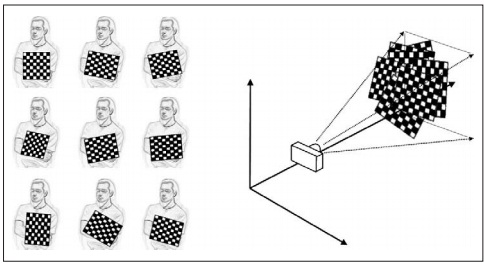
\includegraphics[width=0.8\linewidth]{pics/calibrationMan.png}}
\caption{Процесс гибкого метода калбровка камеры.}
\label{pic:calibrationMan}
\end{figure}

В то же время, данный метод можно применять для вычисления матрицы трансформации изображений. Рассмотрим рисунок~\ref{pic:perspectiveTranform}. Если фиксировать изображения шахматной доски в плоскости левой фигуры, то при удалении искажений мы получим изображение строго перпендикулярное камере. В визуальной одометрии наоборот необходимо отобразить все ключевые точки в плоскости пола. Таким образом, получив матрицу изменения изображения, транспонируем ее и будем применять для нормализованных изображений с целью определить реальное положение ключевых точек кадра на плоскости перемещения. 

\begin{figure}[!h]
\center{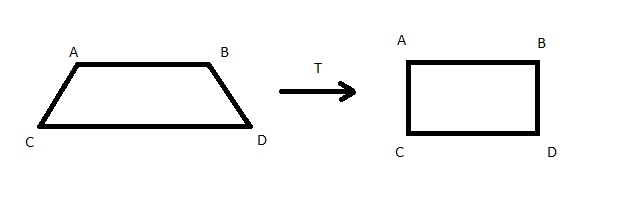
\includegraphics[width=0.8\linewidth]{pics/perspectiveTransform.png}}
\caption{Принцип перспективного преобразования изображений.}
\label{pic:perspectiveTranform}
\end{figure}

После установки необходимого оборудования и его калибровки необходимо согласовать программный интерфейс подсистемы для корректного передачи видеоряда и данных с ИИУ. 
Подсистема ПАОПО предоставляет следующий API:

\begin{verbatim}
PutNewData(Frame currentFrame, Acelleration[] acel,
Rotation[] rotation, callback onResultAvaliable 
[,timestamp  currrentTime])
\end{verbatim}
\begin{itemize}
\item \textbf{\textit{Frame currentFrame}} - очередной кадр; 
\item \textbf{\textit{Acelleration[] acel}} - массив ускорений по осям $oX$, $oY$, $o Z$;
\item \textbf{\textit{Rotation[] rotation}} - массив угловых скоростей вокруг осей $oX$, $oY$, $o Z$; 
\item \textbf{\textit{callback onResultAvaliable}} - функция обработчик результата;
\item \textbf{\textit{timestamp  currrentTime}} - уникальная метка набора данных. Используется для идентификации выходных данных. 
\end{itemize}


Пользователю необходимо реализовать свой обработчик $onResultAvaliable$ и передать ссылку на этот метод в функцию $PutNewData$. По сигнатуре метод должен быть следующим:

\begin{verbatim}
onResultAvaliable(int dx, int dy, int dAngle)
\end{verbatim}

\begin{itemize}
\item \textbf{\textit{int dx}} - перемещение по оси $oX$;
\item \textbf{\textit{int dy}} - перемещение по оси $oY$;
\item \textbf{\textit{int dAngle}} - угол поворота вокруг оси $oZ$.
\end{itemize}


\subsection{Диаргамма взаимодейсвия компонентов}
В ходе работы подсистемы происходит взаимодействие ее модулей между собой и с внешними системами. Диаграмма последовательности такого взаимодействия показана на рисунке~\ref{pic:secquence}.

\afterpage{
\clearpage
%\thispagestyle{empty}
\begin{landscape}
\begin{center}
	\begin{figure}[H]
	\center{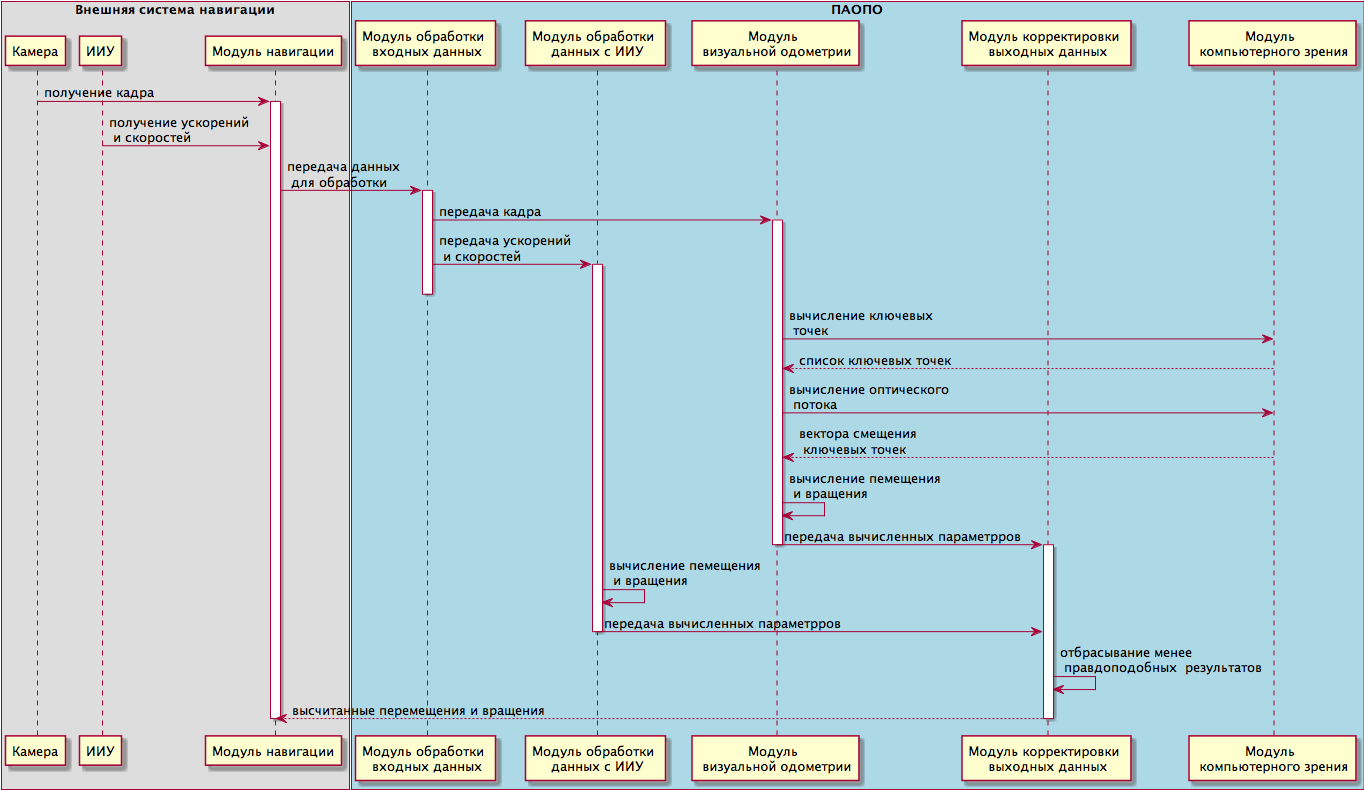
\includegraphics[width=1\linewidth]{pics/sec.png}}
	\caption{Диаграмма последовательности взаимодействия компонентов.}
	\label{pic:secquence}
	\end{figure}
\end{center}
\end{landscape}
\clearpage
}


\subsection{Диаграмма классов подсистемы}
При реализации прототипа рассматриваемой подсистемы был написан программный продукт на  языке Java в программном пакете JetBrains IDEA. В качестве модуля компьютерного зрения использовалась библиотека OpenCV (Open Computer Vision). 
В результате был получен программный продукт состоящий из нескольких классов, связанных между собой. Получившаяся диаграмма классов представлена на рисунке~\ref{pic:classDiagram}.


\afterpage{
\clearpage
%\thispagestyle{empty}
\begin{landscape}
\begin{center}
	\begin{figure}[!htb]
	\center{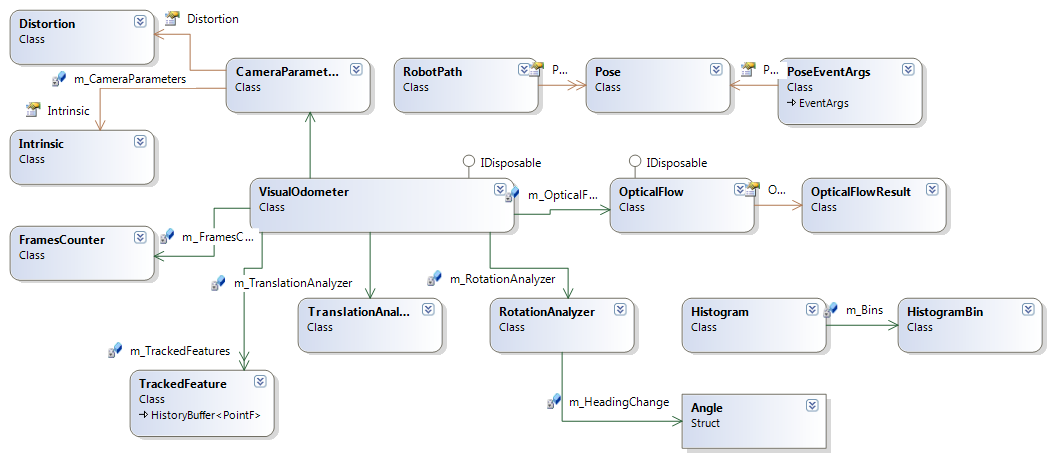
\includegraphics[width=0.9\linewidth]{pics/classDiagram.png}}
	\caption{Диаграмма классов прототипа подсистемы.}
	\label{pic:classDiagram}
\end{figure}
\end{center}
\end{landscape}
\clearpage
}

\subsection{Выбор языка программирования}

В настоящее время существует большое число  языков программирования высокого уровня. Каждый из них обладает своими преимуществами и недостатками. Так как одной из целей создания ПАОПО является создание удобного в интеграции компонента, то выбор языка программирования является важным этапом при реализации подсистемы. 

При этом на выбор языка программирования накладывается ограничение из-за необходимости поддержки библиотеки компьютерного зрения  OpenCV. Согласно документации \cite{OpenCVBook}, OpenCV поддерживает следующие языки программирования:
\begin{itemize}
\item C++;
\item C\#;
\item Java;
\item Python;
\end{itemize}

Проведем выбор среди этих языков программирования методом взвешенных сумм по следующим критериям:
\begin{itemize}
\item кроссплатформенность;
\item производительность;
\item скорость разработки;
\end{itemize}

Сравнение возможных языков по выбранным критериям приведено в таблице~\ref{tab:PLLingvo}.

\begin{table}[!htb]
	\caption{Сравнение языков программирования. Лингвистические оценки.}\label{tab:PLLingvo}
    \centering
	\begin{tabular}{|c|c|c|c|c|}
	\hline 
	Критерий & C++ & C\# & Java & Python \\ 
	\hline 
	Кроссплатформенность & Да & Нет & Да & Да \\ 
	\hline 
	Производительность & Высокая & Средняя & Средняя & Средняя \\ 
	\hline 
	Скорость разработки & Низкая & Высокая & Высокая & Высокая \\ 
	\hline 
	\end{tabular} 
    		
\end{table}

Переведем лингвистические оценки в числовые.

\begin{table}[H]
	\caption{Сравнение языков программирования. Числовые оценки.}
    \centering
	\begin{tabular}{|c|c|c|c|c|}
	\hline 
	Критерий & C++ & C\# & Java & Python \\ 
	\hline 
	Кроссплатформенность  & 1 & 0,4 & 1 & 1 \\ 
	\hline 
	Производительность  & 1 & 0,6 & 0,8 & 0,6 \\ 
	\hline 
	Скорость разработки & 0,3 & 1 & 1 & 0.7 \\ 
	\hline 
	\end{tabular}     		
\end{table}

Учтем весовой коэффициент. Для этого каждому критерию зададим весовой коэффициент, кратный $х$ - минимальному весовому коэффициенту:
\begin{itemize}
\item кроссплатформенность - $2x$;
\item производительность - $3x$;
\item скорость разработки - $1x$;
\end{itemize}

Сумма весовых коэффициентов по всем критериям качества равна 1. тогда:
$$3х + 2х + х = 6х => х = 0,16667$$

Таким образом, можно составить сравнительную таблицу, содержащую количественные и качественные оценки и подсчитать итог, методом взвешенной суммы.
Итоговое сравнение с учетом весового коэффициента и количественных оценок приведены в таблице~\ref{tab:PLitog}.


\begin{table}[!htb]
	\caption{Сравнение языков программирования. Весовой коэффициент и итоговые оценки.}\label{tab:PLitog}
    \centering
	\begin{tabular}{|c|c|c|c|c|c|}
	\hline 
	Критерий & Весовой коэфф. & C++ & C\# & Java & Python \\ 
	\hline 
	Кроссплатформенность & 0,33 & 1 & 0,4 & 1 & 1 \\ 
	\hline 
	Производительность & 0,5 & 1 & 0,6 & 0,8 & 0,6 \\ 
	\hline 
	Скорость разработки  & 0,16667 & 0,3 & 1 & 1 & 0.7 \\ 
	\hline 
	\textbf{Итог}  &  & 0,88 & 0,599 & 0,89 & 0.746 \\ 
	\hline
	\end{tabular}     		
\end{table}




